%pdflatex -shell-escape *.tex
\documentclass{standalone}
\usepackage{amsmath,amsfonts,amssymb}
%
\usepackage{graphicx}
\graphicspath{ {images/} }
%
\usepackage{xcolor}
\pagestyle{empty}
\pagecolor{white}
%
\everymath{\displaystyle}
%
\usepackage{CJKutf8}   %CJKspace
\AtBeginDvi{\input{zhwinfonts}}
%%%
\newcommand{\zh}[1]{\begin{CJK*}{UTF8}{zhsong}#1\end{CJK*}}
\newcommand{\YBao}{\color{red}\zh{源宝爱数学}}
\newcommand{\BT}[1]{\color{red}\zh{#1}\color{black}}
\newcommand{\fTxT}[1]{\text{\zh{#1}}}
%

\immediate\write18{pdflatex test.tex}
\immediate\write18{convert -density 150 -adaptive-resize 480x480 test.pdf test.jpg}
%
%\usepackage{pbox}
%\usepackage{tabularx}
\usepackage{tikz,pgfplots}
% \pgfplotsset{compat=newest}
%\usetikzlibrary{shapes.geometric}
%\pgfplotsset{compat=1.7}
\usetikzlibrary{datavisualization.formats.functions, arrows.meta}
% 
\begin{document}\begin{minipage}[b][14cm][t]{\textwidth}
\begin{center}\large\BT{Test LaTex}\end{center}
%%%
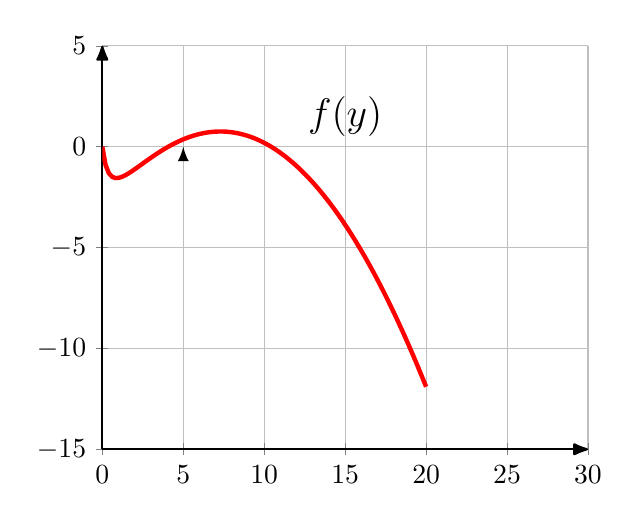
\begin{tikzpicture}
\begin{axis}[scale=0.9, xmin=0, xmax=30, ymin=-15, ymax=5, grid = both,
axis x line=bottom,thick,axis line style={-Latex[round]},
axis y line=left,thick,axis line style={-Latex[round]},
]

\addplot[red, ultra thick] expression[domain=0:20, samples=100]{1.2*x*(1-(x/15))-(4*x)/(0.5+x)};
\node[below,text=black,font=\Large] at (15,3) {$f(y)$};
\draw[-latex](5,0);
\end{axis}
\end{tikzpicture}
% \begin{tikzpicture}
% \begin{axis}[grid=major,axis x line=middle,
%              axis y line=middle,
%              after end axis/.code={
%                \draw[red,->] (axis cs:0,0) -- (axis cs:0.5,0);
%              }]
% \addplot[domain=0:1, no markers] {(x^2)*(3-2*x)};
% \end{axis}
% \end{tikzpicture}

% \begin{tikzpicture}
% \begin{axis}[grid=major,axis x line=middle,
%              axis y line=middle]

% \addplot[domain=0:1, no markers] {(x^2)*(3-2*x)};

% \addplot[] coordinates
%            {(0,0) (0.5,0)};
% \end{axis}
% \end{tikzpicture}
% \begin{tikzpicture}
% \begin{axis}
% \addplot [dash pattern=on 4pt off 1pt on 4pt off 4pt] {x^2};
% \end{axis}
% \end{tikzpicture}
% \begin{tikzpicture}
% \tikzset{myarrow/.style=
%          {sloped,isosceles triangle,anchor=apex,fill=black,inner sep=2pt}}
% \begin{axis}
% \addplot [smooth] {-x^2}
%  node[pos=0.4,myarrow,rotate=180]{} %ok
%  node[pos=0.6,myarrow]{}; %ok

% \addplot[smooth,green] {-x^2+2*x-4}
%  node[pos=0.4,myarrow,rotate=180]{}
%  node[pos=0.6,myarrow]{} %wrong side
%  node[myarrow,fill=red] at (axis cs:4,-12){}; %wrong rotation!
% \end{axis}

% \end{tikzpicture} 
% \begin{figure}  \centering  \begin{tikzpicture}  \begin{axis}[ %  xlabel={x-Achse} ,  
% ylabel={y-Achse},
% ytick=\empty, % That's the trick  ]  \addplot[mark=square*,blue] coordinates {    (1, 1)    (2, 5)    (3, 20)    };  \end{axis}  \end{tikzpicture}  \end{figure}
%%%
% \begin{tikzpicture}
% \begin{axis}[
%     minor x tick num=1,
%     axis lines=middle,    % <--- changed
%     tick label style={font=\scriptsize},
%     ymin=-4.9,ymax=23,
%     xmin=-1,xmax=4.9,
%     xtick={3,4},         % <--- added
%     extra x ticks={1,2}, % <--- added
%     extra x tick style={tick label style={yshift=1mm,anchor=south}},% <--- added
%     x label style={anchor=north east}, % <--- added
%     y label style={anchor=north east}, % <--- added
%     xlabel=$x$,
%     ylabel=$y$
%             ]
% \addplot[blue,smooth,domain=-.5:4,samples=30] {x^3 - 3*x^2 + 1};
% \filldraw [thick,blue] (4,17) circle (1.5pt) node[right,font=\scriptsize] {$(4,17)$}; % <--- added node
% \filldraw [thick,blue] (2,-3) circle (1.5pt) node[below,font=\scriptsize] {$(2,-3)$}; % <--- added node
% \node [right] at (1,20) {$x^3 - 3x^2 + 1$};% <--- added
% \end{axis}
% \end{tikzpicture}
% \begin{tikzpicture}
% \begin{axis}[tick label style={font=\scriptsize},minor x tick num=1, axis y line=middle,axis x line=middle,ymin=-5,ymax=21,xmin=-1,xmax=5,xlabel=$x$,ylabel=$y$]
% \addplot[blue,smooth,domain=-.5:4,samples=30] {x^3 - 3*x^2 + 1}; 
% \filldraw [thick,blue] (axis cs:2,-3) circle (1.5pt);
% \filldraw [thick,blue] (axis cs:4,17) circle (1.5pt); 
% \end{axis}
% \end{tikzpicture}  
% \begin{tikzpicture}
% \begin{axis}
% [
%     title={Contour plot, view from top},
%     view={0}{90}
% ]
% \addplot3[
%     contour gnuplot={levels={0.8, 0.4, 0.2, -0.2}}
% ]
% {sin(deg(sqrt(x^2+y^2)))/sqrt(x^2+y^2)};
% \end{axis}
% \end{tikzpicture}
%%% 
% \begin{tikzpicture}
% \begin{axis}[
%     title=Exmple using the mesh parameter,
%     hide axis,
%     colormap/cool,
% ]
% \addplot3[
%     mesh,
%     samples=50,
%     domain=-8:8,
% ]
% {sin(deg(sqrt(x^2+y^2)))/sqrt(x^2+y^2)};
% \addlegendentry{$\frac{sin(r)}{r}$}
% \end{axis}
% \end{tikzpicture}
%%%
% \begin{tikzpicture}
% \begin{axis}[
% 	x tick label style={
% 		/pgf/number format/1000 sep=},
% 	ylabel=Year,
% 	enlargelimits=0.05,
% 	legend style={at={(0.5,-0.1)},
% 	anchor=north,legend columns=-1},
% 	ybar interval=0.7,
% ]
% \addplot 
% 	coordinates {(2012,408184) (2011,408348)
% 		 (2010,414870) (2009,412156)};
% \addplot 
% 	coordinates {(2012,388950) (2011,393007) 
% 		(2010,398449) (2009,395972)};
% \legend{Men,Women}
% \end{axis}
% \end{tikzpicture}
% \begin{tikzpicture}
% \begin{axis}[
%     title={Temperature dependence of CuSO$_4\cdot$5H$_2$O solubility},
%     xlabel={Temperature}, %[\textcelsius],
%     ylabel={Solubility [g per 100 g water]},
%     xmin=0, xmax=100,
%     ymin=0, ymax=120,
%     xtick={0,20,40,60,80,100},
%     ytick={0,20,40,60,80,100,120},
%     legend pos=north west,
%     ymajorgrids=true,
%     grid style=dashed,
% ]
% \addplot[
%     color=blue,
%     mark=square,
%     ]
%     coordinates {
%     (0,23.1)(10,27.5)(20,32)(30,37.8)(40,44.6)(60,61.8)(80,83.8)(100,114)
%     };
%     \legend{CuSO$_4\cdot$5H$_2$O}
% \end{axis}
% \end{tikzpicture}
%%% 
% \begin{tikzpicture}
% \begin{axis}[
%     axis lines = left,
%     xlabel = $x$,
%     ylabel = {$f(x)$},
% ]
% %Below the red parabola is defined
% \addplot [
%     domain=-10:10, 
%     samples=100, 
%     color=red,
% ]
% {x^2 - 2*x - 1};
% \addlegendentry{$x^2 - 2x - 1$}
% %Here the blue parabloa is defined
% \addplot [
%     domain=-10:10, 
%     samples=100, 
%     color=blue,
%     ]
%     {x^2 + 2*x + 1};
% \addlegendentry{$x^2 + 2x + 1$}
% \end{axis}
% \end{tikzpicture}
%%%
% \begin{tikzpicture}
% \begin{axis}
% \addplot[color=red]{exp(x)};
% \end{axis}
% \end{tikzpicture}
% %Here ends the furst plot
% \hskip 5pt
% %Here begins the 3d plot
% \begin{tikzpicture}
% \begin{axis}
% \addplot3[
%     surf,
% ]
% {exp(-x^2-y^2)*x};
% \end{axis}
% \end{tikzpicture}
%%%
% \begin{tikzpicture}[domain=0:3]
% \begin{axis}[xlabel=Frequency(GHz), ylabel=Output Power(dBm)]
% \addplot[color=blue,only marks]
%   table[x=x,y=y] {
% x         y        
% 100  12.9        
% 130  7.7     
% 140  8
% 144  5     
% 150  6.3 
% 150  12.2 
% 213  -3.2        

% };
% \node[red,above] at (axis cs:102,12.9){\small{'12 MTT}};
% \node[red,below] at (axis cs:104,12.9){\small{65nm CMOS}};

% \node[red,left] at (axis cs:130,7.7){\small{'12 MWCL}};
% \node[red,below left] at (axis cs:130,7.7){\small{0.13$\mu$m CMOS}};

% \end{axis}
% \end{tikzpicture}
%%%
% \begin{tikzpicture}[>=latex]
% %x axis
% \draw[->] (-5,0) -- (5,0) node[below] {$x$};
% \foreach \x in {-4,...,-1,1,2,...,4}
% \draw[shift={(\x,0)}] (0pt,2pt) -- (0pt,-2pt) node[below] {\footnotesize $\x$};
% %y axis
% \draw[->] (0,-5) -- (0,5) node[left] {$y$};
% \foreach \y in {-4,...,-1,1,2,...,4}
% \draw[shift={(0,\y)}] (2pt,0pt) -- (-2pt,0pt) node[left] {\footnotesize $\y$};
% \node[below left] at (0,0) {\footnotesize $0$};
% \end{tikzpicture}
% \begin{tabular}{|l|l|} \hline
%     \pbox{20cm}{This is the first \\ cell} & second \\ \hline
%     3rd & and the last cell \\ \hline
% \end{tabular}
% \begin{tabularx}{\textwidth}{lX}
%     Section:   &  This is my     \newline
%                   long paragraph \\
% \end{tabularx}\\
% %%%                
% \begin{tabular}{|c|c|c|}
% \hline
% here&\vtop{\hbox{\strut top line}\hbox{\strut botline}}&more\\
% \hline
% x&y&z\\
% \hline
% \end{tabular}
%%% 
\end{minipage}\end{document}
